\chapter{Detecting selection on nucleotide polymorphisms}

At this point, we've refined the neutral theory quite a bit. Our
understanding of how molecules evolve now recognizes that some
substitutions are more likely than others, but we're still proceeding
under the assumption that most nucleotide substitutions are neutral or
detrimental. So far we've argued that variation like what Hubby and
Lewontin~\cite{Hubby-Lewontin66,Lewontin-Hubby66} found is not likely
to be maintained by natural selection. But we have strong evidence
that heterozygotes for the sickle-cell allele are more fit than either
homozygote in human populations where malaria is prevalent. That's an
example where selection is acting to maintain a polymorphism, not to
eliminate it. Are there other examples? How could we detect them?

In the 1970s a variety of studies suggested that a polymorphism in the
locus coding for alcohol dehydrogenase in {\it Drosophila
  melanogaster\/} might not only be subject to selection but that
selection may be acting to maintain the polymorphism. As DNA
sequencing became more practical at about the same time,\footnote{It
  was still {\it vastly\/} more laborious than it is now.} population
geneticists began to realize that comparative analyses of DNA
sequences at protein-coding loci could provide a powerful tool for
unraveling the action of natural selection. Synonymous sites within a
protein-coding sequence provide a powerful standard of
comparision. Regardless of

\begin{itemize}

\item the demographic history of the population from which the
  sequences were collected,

\item the length of time that populations have been evolving under the
  sample conditions and whether it has been long enough for the
  population to have reached a drift-migration-mutation-selection
  equilibrium, or

\item the actual magnitude of the mutation rate, the migration rate,
  or the selection coefficients

\end{itemize}

\noindent the synonymous positions within the sequence provide an
internal control on the amount and pattern of differentiation that
should be expected when substitutions.\footnote{Ignoring, for the
  moment, the possibility that there may be selection on codon usage.}
Thus, if we see different patterns of nucleotide substitution at
synonymous and non-synonymous sites, we can infer that selection is
having an effect on amino acid substitutions.

\section*{Nucleotide sequence variation at the {\it Adh\/} locus in
  {\it Drosophila melanogaster}}\index{Drosophila@\textit{Drosophila}!\textit{melanogaster}}\index{alcohol dehydrogenase}\index{Adh}

Kreitman~\cite{Kreitman83} took advantage of these ideas to provide
additional insight into whether natural selection was likely to be
involved in maintaining the polymorphism at {\it Adh\/} in {\it
  Drosophila melanogaster}. He cloned and sequenced 11 alleles at this
locus, each a little less than 2.4kb in length.\footnote{Think about
  how the technology has changed since then. This work represented a
  major part of his Ph.D. dissertation, and the results were published
  as an article in {\it Nature}.} If we restrict our attention to the
coding region, a total of 765bp, there were 6 distinct sequences that
differed from one another at between 1 and 13 sites. Given the
observed level of polymorphism within the gene, there should be 9 or
10 amino acid differences observed as well, but only one of the
nucleotide differences results in an amino acid difference, the amino
acid difference associated with the already recognized electrophoretic
polymorphsim. Thus, there is significantly less amino acid diversity
than expected if nucleotide substitutions were neutral, consistent
with my assertion that most mutations are deleterious and that natural
selection will tend to eliminate them.\index{Adh!purifying selection}
In other words, another example of the ``sledgehammer
principle.''\index{sledgehammer principle}

Does this settle the question? Is the {\it Adh\/} polymorphism another
example of allelic variants being neutral or selected against? Would I
be asking these questions if the answer were ``Yes''?

\subsection*{Kreitman and Aguad{\'e}}

A few years after Kreitman~\cite{Kreitman83} appeared, Kreitman and
Aguad{\'e}~\cite{Kreitman-Aguade86} published an analysis in which
they looked at levels of nucleotide diversity in the {\it Adh\/}
region, as revealed through analysis of RFLPs, in {\it
  D. melanogaster\/} and the closely related {\it D. simulans}. Why
the comparative approach? Well, Kreitman and Aguad{\'e} recognized
that the neutral theory of molecular evolution makes two predictions
that are related to the underlying mutation rate:

\begin{itemize}

\item If mutations are neutral, the substitution rate is equal to the
  mutation rate.

\item If mutations are neutral, the diversity within populations
  should be about $4N_e\mu/(4N_e\mu + 1)$.

\end{itemize}

\noindent Thus, if variation at the {\it Adh\/} locus in {\it
  D. melanogaster\/} is selectively neutral, the amount of divergence
between {\it D. melanogaster\/} and {\it D. simulans\/} should be
related to the amount of diversity within each. What they found
instead is summarized in Table~\ref{table:ka}.\index{Adh!balancing selection}\index{diversity-divergence}

\begin{table}
\begin{center}
\begin{tabular}{l|ccc}
\hline\hline
         & 5' flanking & {\it Adh\/} locus & 3' flanking \\
\hline
Diversity$^1$ \\
\quad Observed & 9     & {\bf 14}   & 2    \\
\quad Expected & 10.8  & 10.8 & 3.4  \\
Divergence$^2$ \\
\quad Observed & 86    & 48   & 31   \\
\quad Expected & 55    & {\bf 76.9} & 33.1 \\
\hline
\multicolumn{4}{l}{$^1$Number of polymorphic sites within {\it
         D. melanogaster\/}} \\
\multicolumn{4}{l}{$^2$Number of nucleotide differences between {\it
         D. melanogaster\/} and {\it D. simulans}}
\end{tabular}
\end{center}
\caption{Diversity and divergence in the {\it Adh\/} region of {\it
    Drosophila}~(from~\cite{Kreitman-Aguade86}).}\label{table:ka}
\end{table}

Notice that there is substantially less divergence at the {\it Adh\/}
locus than would be expected, based on the average level of divergence
across the entire region. That's consistent with the earlier
observation that most amino acid substitutions are selected
against. On the other hand, there is {\it more\/} nucleotide diversity
within {\it D. melanogaster\/} than would be expected based on the
levels of diversity seen in across the entire region. What gives?

Time for a trip down memory lane. Remember something called
``coalescent theory?'' It told us that for a sample of neutral genes
from a population, the expected time back to a common ancestor for all
of them is about $4N_e$ for a nuclear gene in a diploid
population. That means there's been about $4N_e$ generations for
mutations to occur. Suppose, however, that the electrophoretic
polymorphism were being maintained by natural selection. Then we might
well expect that it would be maintained for a lot longer than $4N_e$
generations. If so, there would be a lot more time for diversity to
accumulate. Thus, the excess diversity could be accounted for if there
is balancing selection at ADH.\index{coalescent!balancing selection}

\subsection*{Kreitman and Hudson}

Kreitman and Hudson~\cite{Kreitman-Hudson91} extended this approach by
looking more carefully within the region to see where they could find
differences between observed and expected levels of nucleotide
sequence diversity. They used a ``sliding window'' of 100 silent base
pairs in their calculations. By ``sliding window'' what they mean is
that first they calculate statistics for bases 1-100, then for bases
2-101, then for bases 3-102, and so on until they hit the end of the
sequence. It's rather like walking a chromosome for QTL mapping, and
the results are rather pretty~(Figure~\ref{fig:kh}). 

\begin{figure}
\begin{center}
\resizebox{!}{6cm}{\includegraphics{kreitman-hudson.eps}}
\end{center}
\caption{Sliding window analysis of nucleotide diversity in the {\it
    Adh\/}-{\it Adh-dup} region of {\it Drosophila melanogaster}. The
  arrow marks the position of the single nucleotide substitution that
  distinguishes {\it Adh-F\/} from {\it
    Adh-S\/}~(from~\cite{Kreitman-Hudson91})}\label{fig:kh}
\end{figure}

To me there are two particularly striking things about this
figure. First, the position of the single nucleotide substitution
responsible for the electrophoretic polymorphism is clearly
evident. Second, the excess of polymorphism extends for only a 200-300
nucleotides in each direction. That means that the rate of
recombination {\it within\/} the gene is high enough to randomize the
nucleotide sequence variation farther away.\footnote{Think about what
  that means for association mapping. In organisms with a large
  effective population size, associations due to physical linkage may
  fall off {\it very\/} rapidly, meaning that you would have to have a
  {\it very\/} dense map to have a hope of finding associations.}

\section*{Detecting selection in the human genome}

I've already mentioned the HapMap project~\cite{HapMap-2007}, a
collection of genotype data at roughly 3.2M SNPs in the human
genome. The data in phase II of the project were collected from four
populations:

\begin{itemize}

\item Yoruba (Ibadan, Nigeria)

\item Japanese (Tokyo, Japan)

\item Han Chinese (Beijing, China)

\item ancestry from northern and western Europe (Utah, USA)

\end{itemize}

We expect genetic drift to result in allele frequency differences
among populations, and we can summarize the extent of that
differentiation at each locus with $F_{ST}$. If all HapMap SNPs are
selectively neutral,\footnote{And unlinked to sites that are under
  selection.} then all loci should have the same $F_{ST}$ within the
bounds of statistical sampling error and the evolutionary sampling due
to genetic drift. A scan of human chromosome 7 reveals both a lot of
variation in individual-locus estimates of $F_{ST}$ and a number of
loci where there is substantially more differentiation among
populations than is expected by
chance~(Figure~\ref{fig:low-res-SNP}). At very fine genomic scales we
can detect even more outliers~(Figure~\ref{fig:high-res-SNP}),
suggesting that human populations have been subject to divergent
selection pressures at many different loci~\cite{Guo-etal-2009}.\index{F-statistics@$F$-statistics!outliers}

\begin{figure}
\begin{center}
\resizebox{\textwidth}{!}{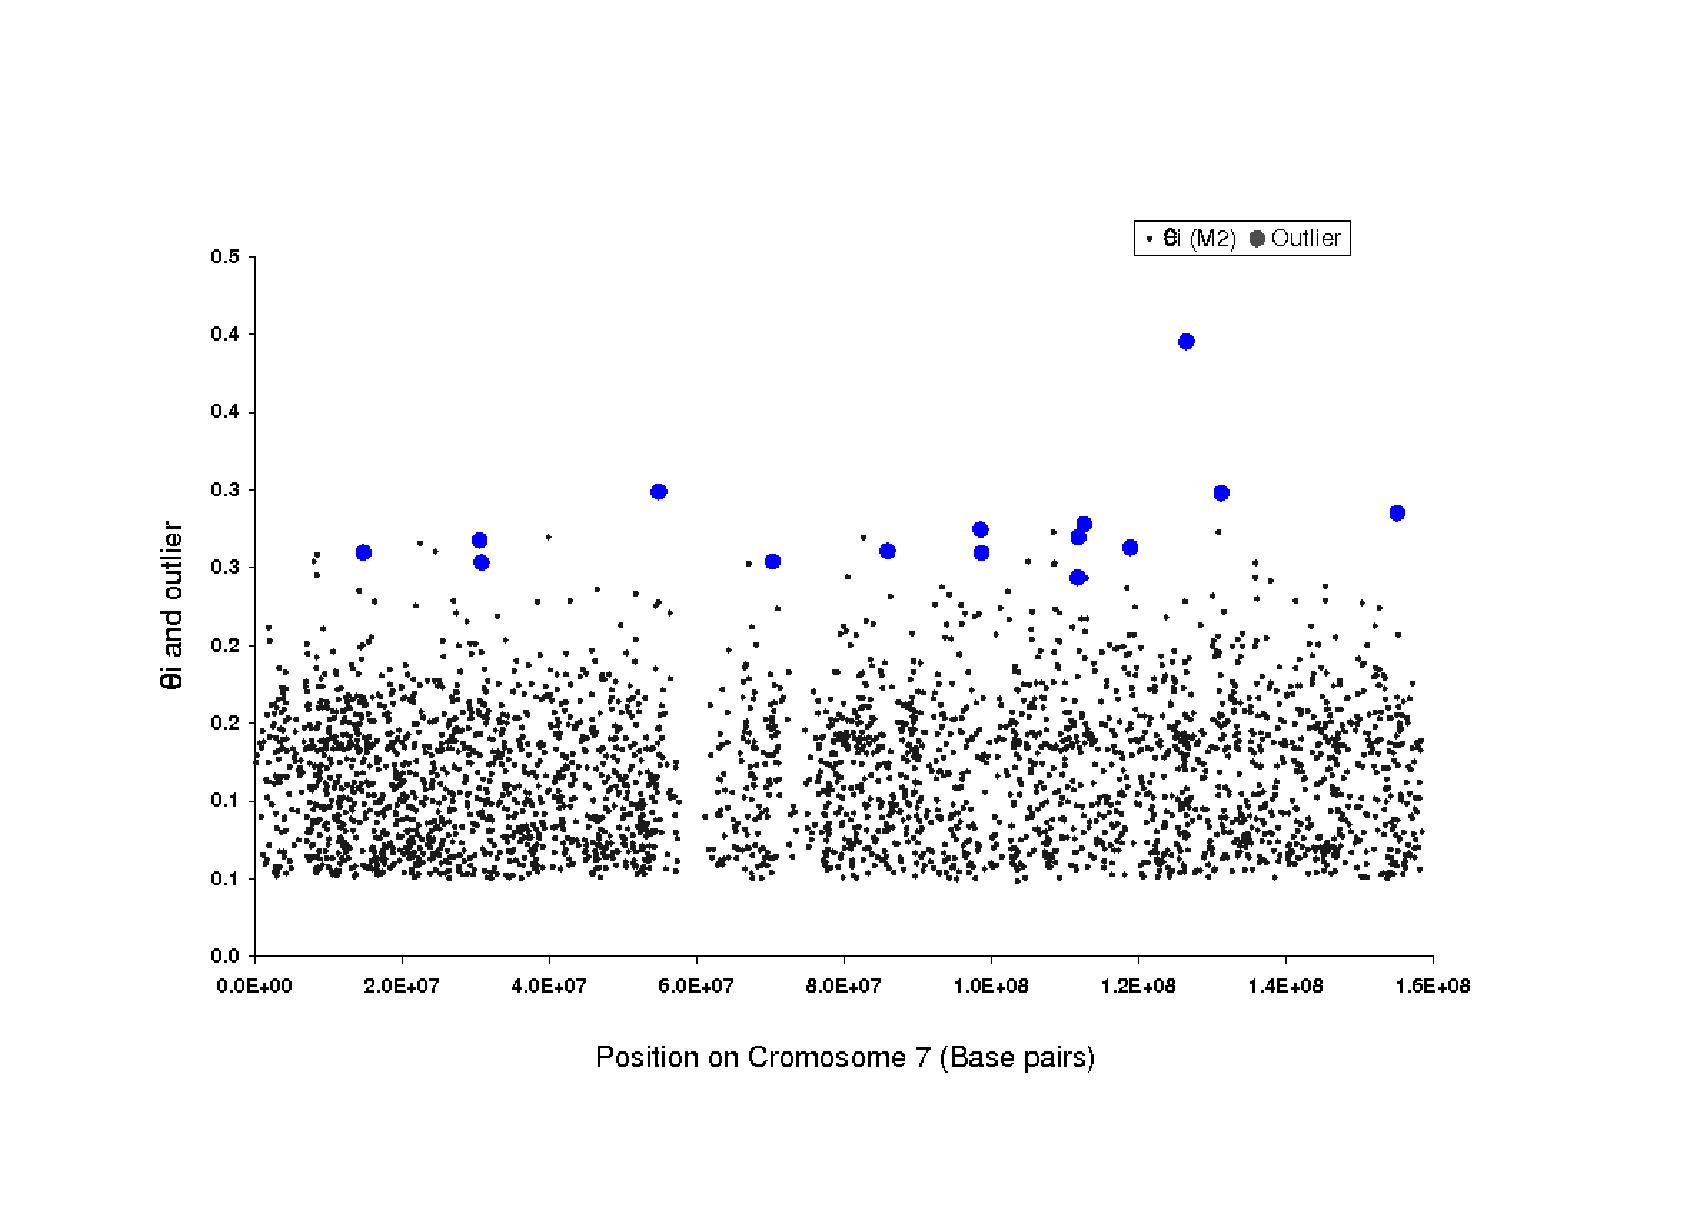
\includegraphics{outlier.eps}}
\end{center}
\caption{Single-locus estimates of $F_{ST}$ along chromosome 7 in the
  HapMap data set. Blue dots denote outliers. Adjacent SNPs in this
  sample are separated, on average, by about
  52kb. (from~\cite{Guo-etal-2009})}\label{fig:low-res-SNP}
\end{figure}

\begin{figure}
\begin{center}
\resizebox{\textwidth}{!}{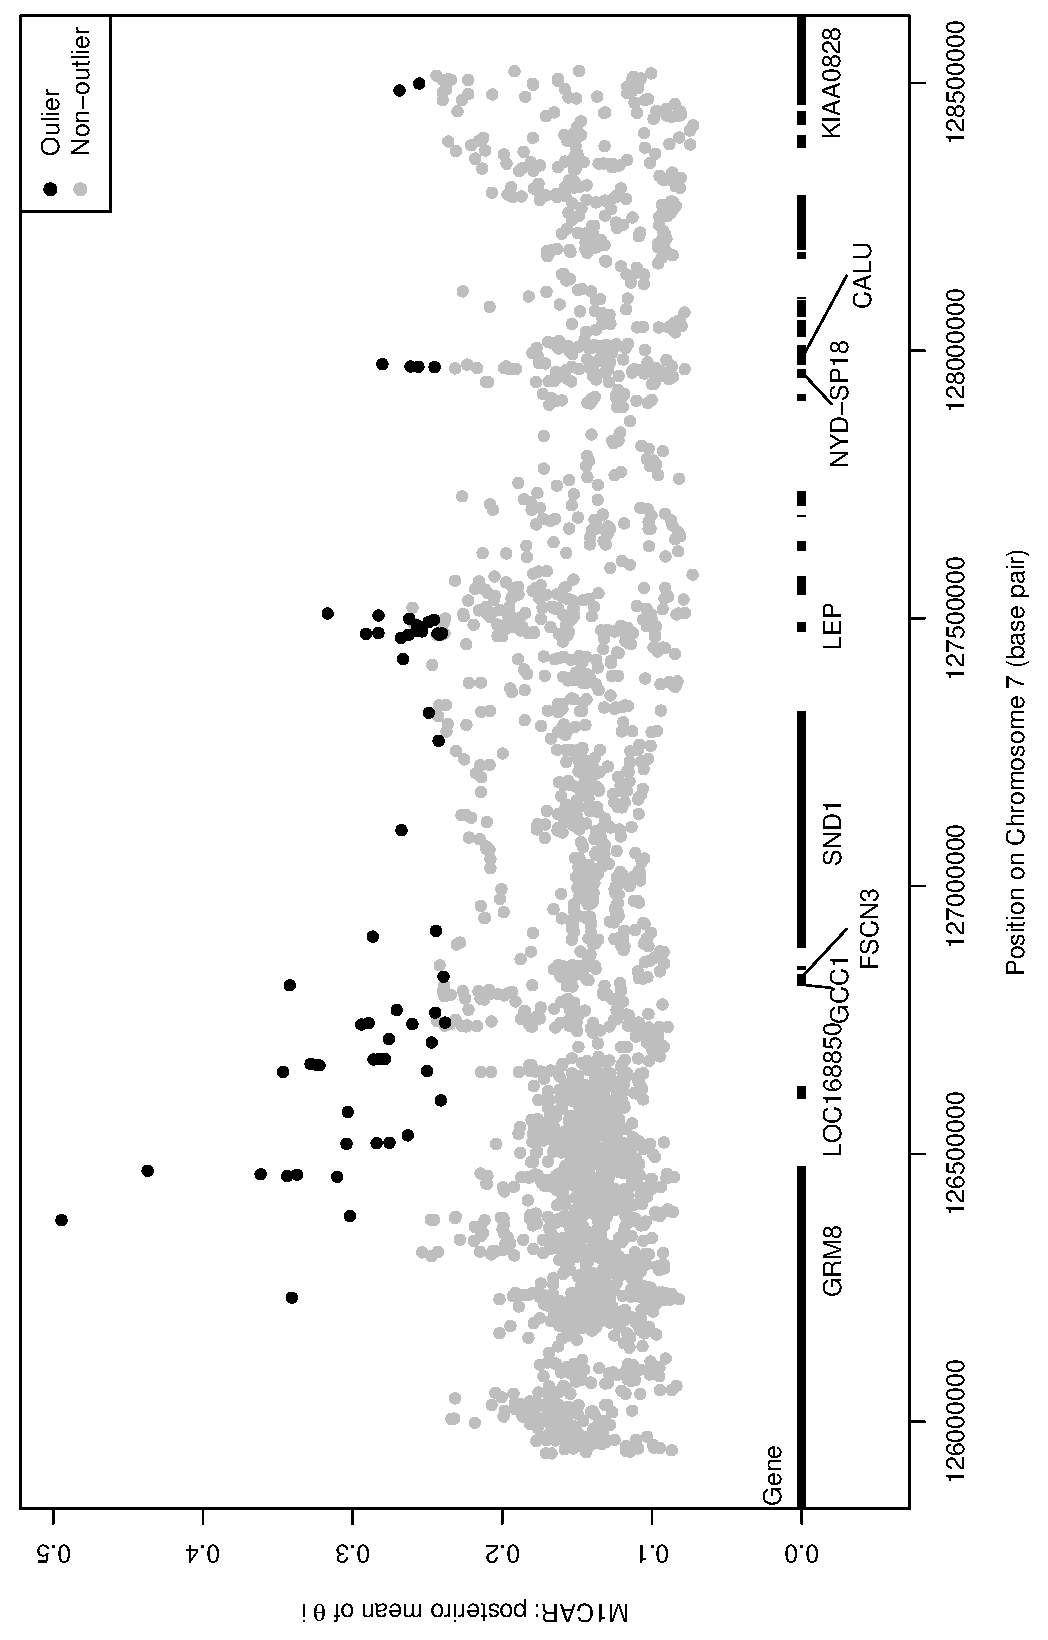
\includegraphics[angle=270]{outlier-high.eps}}
\end{center}
\caption{Single-locus estimates of $F_{ST}$ along a portion of
  chromosome 7 in the HapMap data set. Black dots denote
  outliers. Solid bars refert to previously identified genes. Adjacent
  SNPs in this sample are separated, on average, by about
  1kb. (from~\cite{Guo-etal-2009})}\label{fig:high-res-SNP}
\end{figure}

